%======================================================================
\section{Del modelo continuo al problema de optimización}\label{sec:numerica}
%======================================================================
El ROM es un sistema de ecuaciones diferenciales en tiempo continuo, y el optimizador
trabaja con un número finito de variables. Esta sección explica cómo se pasa de uno a otro:
primero se \emph{discretiza} el tiempo, y luego se decide cómo entran esas ecuaciones
discretas en el problema de optimización.

\subsection{Integrar una ecuación diferencial: Euler explícito e implícito}
Para $\dot x=f(x)$ con paso $h$, los dos esquemas más simples son:
\[
\text{Euler explícito:}\quad x_k=x_{k-1}+h\,f(x_{k-1}),\qquad
\text{Euler implícito:}\quad x_k=x_{k-1}+h\,f(x_k).
\]
El explícito usa la pendiente del punto conocido y da $x_k$ directamente. El implícito usa la
pendiente del punto nuevo, así que $x_k$ aparece a ambos lados y hay que resolver una ecuación,
normalmente con Newton, en cada paso. La ventaja del implícito es la estabilidad.

\begin{proposicion}[Estabilidad en la ecuación de prueba]\label{prop:estab}
Para $\dot x=\lambda x$ con $\lambda<0$, cuya solución exacta decae, Euler explícito produce
$x_k=(1+h\lambda)^kx_0$, que decae sólo si $h<2/|\lambda|$. Euler implícito produce
$x_k=(1-h\lambda)^{-k}x_0$, que decae para todo $h>0$.
\end{proposicion}
\begin{proof}
Explícito: $x_k=x_{k-1}+h\lambda x_{k-1}=(1+h\lambda)x_{k-1}$, y $|1+h\lambda|<1$ si y sólo si
$0<h|\lambda|<2$. Implícito: $x_k=x_{k-1}+h\lambda x_k$, así que
$x_k=x_{k-1}/(1-h\lambda)$, y como $1-h\lambda=1+h|\lambda|>1$, el factor es menor que uno para
cualquier $h>0$.
\end{proof}
\noindent Un esquema con esa propiedad para todo $\lambda$ de parte real negativa se llama
\emph{A-estable}~\cite{hairer1996}. La figura~\ref{fig:stiff} lo muestra en un ejemplo
ilustrativo: con $h\lambda=2.5$, Euler explícito oscila y explota, mientras que Euler implícito
sigue la solución.

\begin{figure}[H]\centering
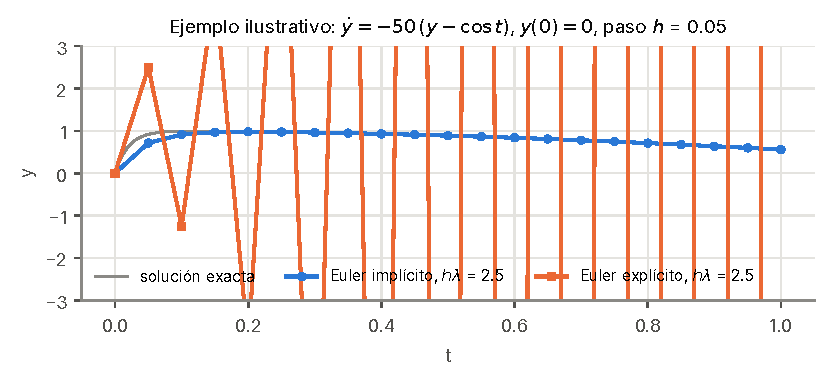
\includegraphics[width=\linewidth]{figures/did_stiff.pdf}
\caption{Ejemplo ilustrativo de rigidez: $\dot y=-50\,(y-\cos t)$, $y(0)=0$, con paso $h=0.05$.
La solución se acerca a $\cos t$ en una escala de tiempo de $1/50$~s. Con $h\lambda=2.5>2$,
Euler explícito (naranja) es inestable; Euler implícito (azul) es estable con el mismo paso.}
\label{fig:stiff}
\end{figure}

\subsection{La rigidez del ROM}
Un sistema es \emph{rígido} cuando tiene modos con escalas de tiempo muy distintas. Para
$\dot x=f(x)$, las escalas son los inversos de los valores propios del jacobiano
$A=\partial f/\partial x$. La figura~\ref{fig:eigs} muestra los 17 valores propios del ROM en
las dos consultas:
\begin{itemize}
  \item el modo más rápido, $\lambda\approx-1.7\cdot10^3$~s$^{-1}$, es la cinética neutrónica
        inmediata, con una escala de $0.6$~ms;
  \item los de los precursores y las temperaturas van de $-20$ a $-0.01$~s$^{-1}$;
  \item hay un valor propio \emph{exactamente cero}: el inventario $\Delta M$, que es un
        integrador puro de los caudales.
\end{itemize}
Con $\Delta t=0.5$~s, Euler explícito sería inestable en los cinco modos con
$|\lambda|>2/\Delta t=4$~s$^{-1}$ (proposición~\ref{prop:estab}). Para ser estable necesitaría
un paso de $2/1700\approx1.2$~ms, unas 400 veces menor. Euler implícito permite el paso de
0.5~s del controlador, y por eso Simulink lo usa.

\begin{figure}[H]\centering
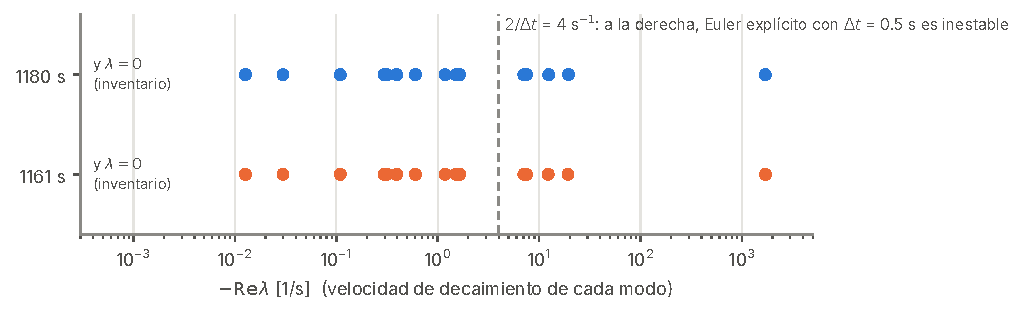
\includegraphics[width=\linewidth]{figures/did_eigs.pdf}
\caption{Valores propios del jacobiano del ROM en las dos consultas, en escala logarítmica de
la tasa de decaimiento. Cubren cinco órdenes de magnitud: el sistema es rígido. La línea
discontinua marca el límite de estabilidad de Euler explícito con el paso del controlador.}
\label{fig:eigs}
\end{figure}

\subsection{Euler implícito convergido y \code{ode1be}}
Resolver exactamente la ecuación implícita en cada paso exige iterar Newton hasta la
convergencia: es \textbf{Euler implícito convergido} (BE). Simulink, con el integrador
\code{ode1be}, hace \emph{una sola} iteración de Newton desde el punto anterior:
\[
x_k=x_{k-1}+\big(I-\Delta t\,A(x_{k-1})\big)^{-1}\Delta t\,f(x_{k-1},d_k,u_k).
\]
Las dos versiones difieren poco: el error está en el transitorio inicial de cada simulación y no
en el horizonte (sección~\ref{sec:replica}). El problema monolítico usa BE, porque es una
ecuación exacta que puede imponerse como restricción. La sección~\ref{sec:certificacion}
comprueba que el óptimo no cambia al usar \code{ode1be}.

\subsection{Cómo entra la dinámica en la optimización}
Una vez discretizado, P0 tiene los caudales $u_1,\dots,u_K$ como decisión y los estados
$x_1,\dots,x_K$ determinados por ellos. Hay dos maneras de plantearlo
(figura~\ref{fig:shooting})~\cite{betts2010,biegler2010}:

\begin{figure}[H]\centering
\resizebox{\linewidth}{!}{%
\begin{tikzpicture}[
  bx/.style={draw=ink, line width=0.6pt, rounded corners=2pt, fill=white, align=center, font=\small, minimum height=11mm, text width=30mm},
  op/.style={draw=accent, line width=0.6pt, rounded corners=2pt, fill=soft, align=center, font=\small, minimum height=11mm, text width=32mm},
  arr/.style={-{Stealth[length=2mm]}, line width=0.6pt, draw=ink},
  lab/.style={font=\footnotesize, text=black!70, align=center}]
\node[font=\small\bfseries, text=ink] at (3.6,2.1) {Disparo simple (caja negra)};
\node[op] (o1) at (0,0) {optimizador\\propone $u$};
\node[bx] (s1) at (4.4,0) {simulador:\\$x_1,\dots,x_K=\mathcal S(x_0,u)$};
\node[bx] (j1) at (8.4,0) {costo\\$J(u)$};
\draw[arr] (o1) -- (s1); \draw[arr] (s1) -- (j1);
\draw[arr] (j1.south) -- ++(0,-0.6) -| node[lab, pos=0.25, below]{sólo un número} (o1.south);
\node[font=\small\bfseries, text=ink] at (14.2,2.1) {Transcripción directa (monolítica)};
\node[op, text width=56mm, minimum height=24mm] (o2) at (14.2,0) {un solo problema:\\[2pt]
  $\min\limits_{u,\,x}\ J(x,u)$\\[2pt]
  s.a.\ $x_k-x_{k-1}-\Delta t\,f(x_k,d_k,u_k)=0$\\ para $k=1,\dots,K$};
\node[lab] at (14.2,-1.65) {estados y controles son incógnitas;\\la dinámica es un conjunto de restricciones};
\end{tikzpicture}}
\caption{Dos formas de poner la dinámica en un problema de optimización. Izquierda: el
optimizador sólo ve los controles, y cada evaluación del costo es una simulación completa.
Derecha: estados y controles son variables del mismo problema, y las ecuaciones del modelo son
restricciones.}
\label{fig:shooting}
\end{figure}

\paragraph{Disparo simple.} Las únicas variables son los controles. Para evaluar el costo se
simula todo el horizonte. Es lo que hacen LJ y GA, sin derivadas. También puede hacerse con
derivadas, propagándolas a través de la simulación (\emph{espacio reducido}). El problema tiene
pocas variables, pero cada evaluación es costosa, y un error al inicio del horizonte se propaga
a todo el resto.

\paragraph{Transcripción directa simultánea.} Los estados también son variables, y la
dinámica discretizada entra como restricciones de igualdad, llamadas \emph{defectos}. El
problema es más grande (aquí, 519 variables), pero tiene ventajas decisivas:
\begin{itemize}
  \item cada restricción enlaza sólo dos instantes consecutivos, así que las matrices son
        \emph{dispersas} y se factorizan en tiempo casi lineal en $K$;
  \item las derivadas de cada restricción son locales y se obtienen con exactitud;
  \item el optimizador no necesita que la trayectoria sea factible en cada iteración, lo que
        ayuda con dinámicas rígidas o inestables.
\end{itemize}
Una variante intermedia, el \emph{disparo múltiple}, divide el horizonte en tramos simulados y
une sus extremos con restricciones~\cite{bock1984}. En este documento se llama
\textbf{formulación monolítica} a la transcripción directa: el simulador y el optimizador quedan
fusionados en un solo problema.

\subsection{Escalado}
Las variables del ROM van de $10^3$ (temperaturas) a $10^{16}$ (precursores). Si se usan tal cual,
las matrices de Newton quedan mal condicionadas: sus elementos difieren en muchos órdenes de
magnitud, y el redondeo destruye la precisión. Por eso cada estado se escribe como $x_j=S_jz_j$,
con $S_j=\max(|x_{0,j}|,1)$, y el optimizador trabaja con $z$, cuyas componentes son de orden uno.

\takeaway{\textbf{Para recordar.} El ROM es rígido, y por eso se integra con Euler implícito,
que es estable con el paso de 0.5~s. La formulación monolítica no simula para evaluar el
costo: escribe cada paso de Euler implícito como una restricción, de modo que estados y controles
se optimizan juntos, con derivadas exactas y matrices dispersas.}
